\chapter{Fresnel Simulation Toolbox: applications}
\markboth{\MakeUppercase{Fresnel Simulation Toolbox: applications}}{}
\label{chap:fresnel2}
\section{Introduction}
This chapter will describes in details the performance of the different free space propagation operators described in the previous chapter. Some examples of how they can be used to simulate of an optical system will also be presented. Particular attention will be given to the differences between the different operators in terms of performance and signal to noise ratio.
It will also be largely described how to simulate partially coherent light. An original method to simulate both spatial and temporal coherence will be presented. Results form the numerical simulations will also be presented to support the theoretical model and to optimise the parameters.
In future developments of this work could be interesting to evaluate the performances of these methods analytically. But for the nature of this work is it enough to evaluate those performances using the simulations.
\section{Performances of the Angular Spectrum Methods}
 \label{sec:perfAS}
 To evaluate the differences in resolution of the three variants of the angular spectrum methods, normal Angular spectrum (AS), Band Limited Angular Spectrum (BL), and Corrected Band Limited Angular Spectrum (CBL) presented in chapter \ref{chap:fresnel}, a simulation has been implemented consisting of a free space propagation of a constant input field with a circular pupil of diameter 5 mm, sampled with a resolution of 3000 $\times$ 3000 pixels with a sampling window of 1 cm. The propagation distances \textit{z} varied from 1 m to 10 m. The wavelength used was of 633 nm, corresponding to the red Helium-Neon Laser. Performances have been evaluated experimentally through the simulations.\\ 
 The setup simulated is shown in figure \ref{fig:setup111}.
  \begin{figure}[h]
  	\begin{center}
  		\begin{tabular}{c}
  			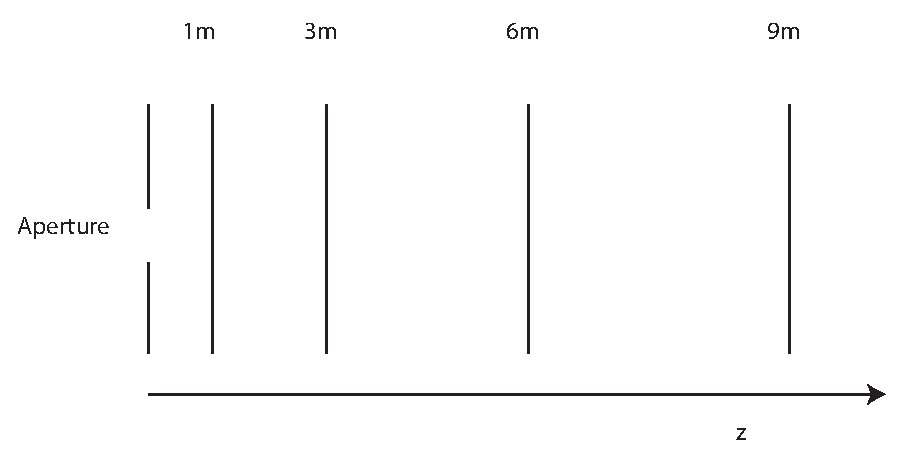
\includegraphics[height=6cm]{perf1.eps}
  		\end{tabular}
  	\end{center}
  	 	\caption	{ \label{fig:setup111} 
  	 		Positions of the plane where the optical field has been sampled with respect to the aperture. }
  	 \end{figure} 
 Results are shown in figure \ref{fig:methods} where the cross section of the diffraction patterns are shown. 
 The BL method shown in the central column gives smooth diffraction patterns. Increasing the propagation distance however leads to the intensity profile losing part of the information because of the excessive low pass filtering on the propagation transfer function, leading the complete loss of the diffraction fringes. A comparison with the AS can be seen in figure \ref{fig:methods}, where the diffraction fringes are presents with the superimposition of the noise due to aliasing in the transfer function sampling. This affects the resolution of the diffraction pattern and the signal to noise ratio (SNR) drops with \textit{z} as shown in figure \ref{fig:SNR1}.The CBL method gives a good noise reduction without losing the original signal shape as explained in section \ref{sec:angular3} and as it is shown in figure \ref{fig:methods} on the far right column. Fringes are clearly present in the diffraction pattern even for large propagation distances and the noise is removed. \\
 In figure figure \ref{fig:SNR1} the SNR of the diffraction patterns in figure \ref{fig:methods} is plotted as a function of the propagation distance for the three examined cases. The BL method gives a better SNR especially for short propagation distances, where the bandwidth of the transfer function is not low pass filtering the signal yet, but only avoiding the aliasing. Its values remains in general above the SNR of the CBL method (almost 15dB), even in the case of large propagation distances. This is due to the excessive smoothing action that leads to the loss of resolution. On the other hand without any bandwidth limitation, AS, green line, the aliasing generated noise becomes dominant for long propagation distances and the SNR approaches the 0 dB value. The best results in terms of resolution and noise reduction are given by the corrected BL method where the information on the diffraction is retained entirely.
 \begin{figure}[H]
 	\begin{center}
 		\begin{tabular}{c}
 			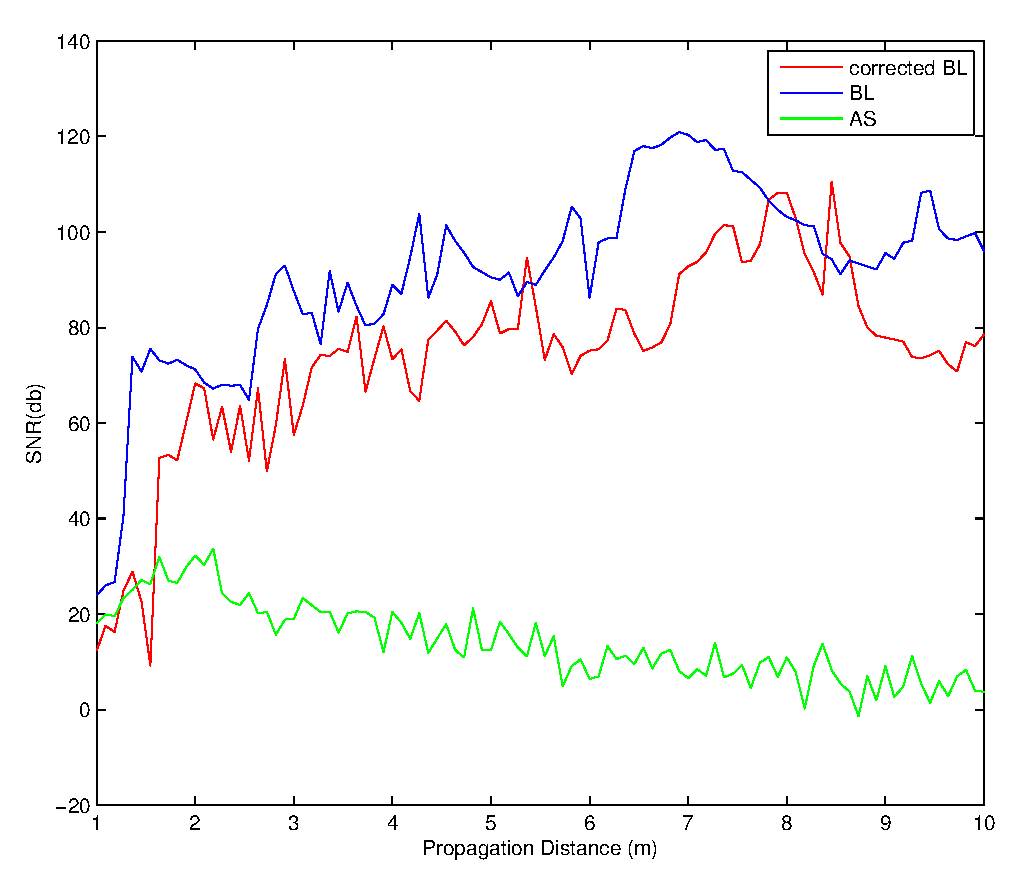
\includegraphics[height=12cm]{SNR_com.eps}
 		\end{tabular}
 	\end{center}
 	\caption	{ \label{fig:SNR1} 
 		Sampling of the  Signal to Noise ratio (SNR) at various values of the propagation distances for the three propagation methods seen in section \ref{sec:angular 2}. The lines are just joining the sampled points and does not represent a model. The BL and the corrected BL methods improve the SNR, that instead drops as the propagation distance increases when the AS method is used. }
 \end{figure}
e 
 \begin{figure}[H]
 	\begin{center}
 		\begin{tabular}{c}
 			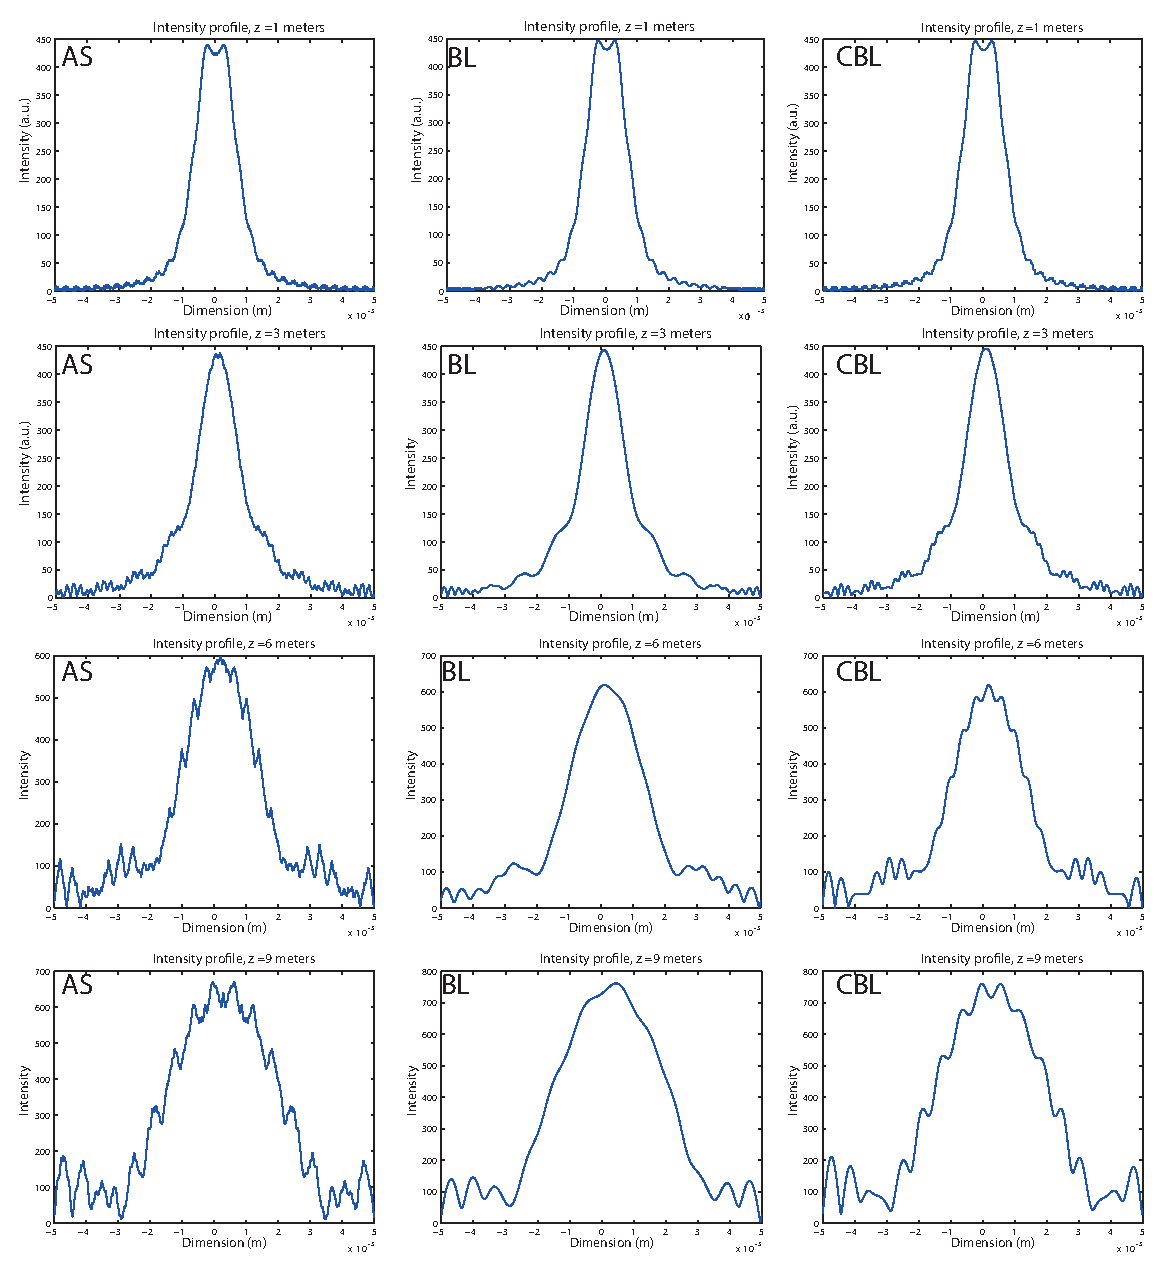
\includegraphics[height=15cm]{methods1.eps}
 		\end{tabular}
 	\end{center}
 	\caption{ \label{fig:methods} 
 		Comparison of the performances of the three angular spectrum propagation operator. Diffraction patterns of a 5mm pupil obtained by the simulations. On the left column are shown diffraction pattern cross section obtained using the angular spectrum method (AS). In the central column the pattern for the same propagation distances have been obtained using the band limited method (BL) and in the right column the same patterns have been obtained using the correct band limited method (corrected BL). }
 \end{figure}
 
 \section{Comparison between the Free Space Propagation Operators}
 \label{sec:comp}
	 In this section the differences in performance between the Fresnel approximation and the angular spectrum of plane waves approach will be shown with particular attention to the computational time required by the different methods, the optical resolution and the error. Results will be used to evaluate the characteristic of the different propagation operators. These results differ from the ones obtained in section \ref{sec:perfAS} since the simulations in this case involve the whole imaging system including the lens and not only the free space propagation.
	 \subsection{Description of the System}
	 \label{sec:system}
	 The system simulated is a simple imaging system composed of a single lens with focal length $f=158mm$, in a \textit{2f} configuration, as shown in figure \ref{fig:2f}. The field of view is a square of $1cm \times 1cm$, and the resolution of the input field is $2000 \times 2000$ pixels. The aperture of the lens is $D=5mm$ and its f number, defined as:
	 \begin{equation}
	 \label{eq:fnum}
		F_{\#}=\dfrac{z}{D}
	 \end{equation}
	 is equal to $F_{\#}=63$, where z is the distance from the lens to the image plane, that in a 2f configuration is equal to $z=2f=316mm$.
	 \begin{figure}[h]
	 	\begin{center}
	 		\begin{tabular}{c}
	 			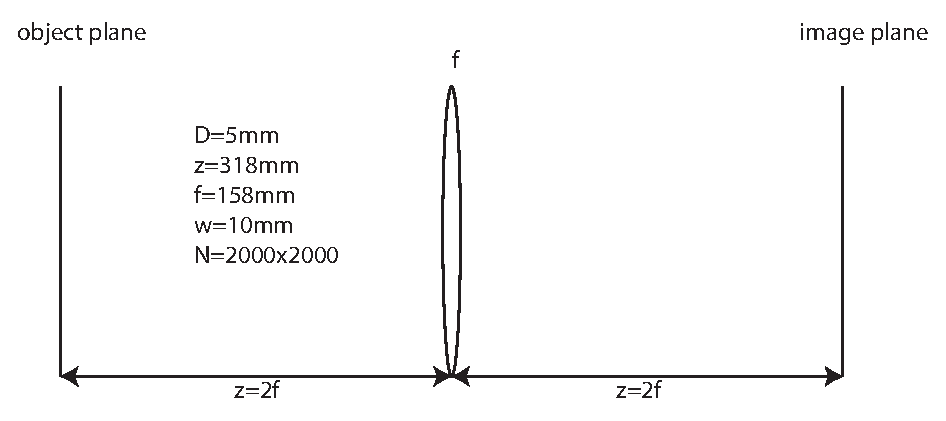
\includegraphics[height=5cm]{C:/Users/Massimo/Documents/Thesis/Thesis_PhD/2f.eps}
	 		\end{tabular}
	 	\end{center}
	 	\caption{ \label{fig:2f} 
	 		Schematic of the 2f system simulated. f is the focal length, z the propagation distances, D is the aperture of the lens, w the field of view and N the sampling resolution. }
	 \end{figure} 
	 The optical cut-off frequency of this system is given by the relation \cite{goodman2005introduction}:
	 \begin{equation}
	 \label{eq:cutoff}
	 \nu_{co}=\dfrac{1}{\lambda F_{\#}}
	 \end{equation} 
	 The object was illuminated with monochromatic light of wavelength $\lambda=633nm$, therefore the cut-off frequency was $\nu_{co}=2.5\cdot10^4 cycles/m$.
	 \subsection{Image of a Point Source}
	 The first experiment simulated is the image of a point source, realized with a pinhole of $10 \mu m$ of diameter placed at the object plane indicated in figure \ref{fig:2f}. The image has been taken using four different methods to propagate the light into the system. Those are:
	 \begin{itemize}
	 	\item Multi step Fresnel method (MSF), section\ref{sec:fresnelmulti}
	 	\item Angular spectrum method (AS), section \ref{sec:angular}
	 	\item Band Limited Angular Spectrum method (BL), section \ref{sec:angular 2}
	 	\item corrected Band Limited Angular Spectrum method (CBL), section \ref{sec:angular3}
	 		 \end{itemize}
The impulse response for a point source as input will be computed using each of these methods.\\
 The sequence of operators used to simulate the system is shown in figure \ref{fig:sequence2} \\
	 \begin{figure}[H]
	 	\begin{center}
	 		\begin{tabular}{c}
	 			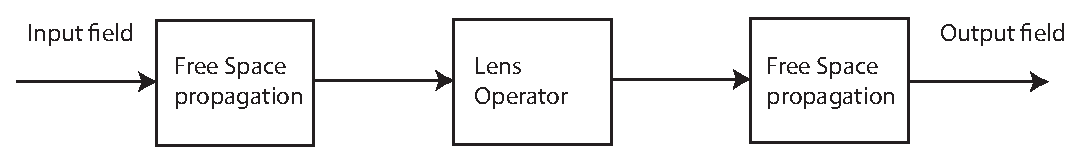
\includegraphics[height=1.8cm]{C:/Users/Massimo/Documents/Thesis/Thesis_PhD/imagesystem.eps}
	 		\end{tabular}
	 	\end{center}
	 	\caption{ \label{fig:sequence2} 
	 		Operator sequence for the 2f system. }
	 \end{figure} 
	 
	In the assumption of having a lens with a circular aperture and no aberrations, the impulse response of an optical system is an Airy Disk, that is the Fourier transform of the pupil of the system at the image plane. The fact that the theoretical output of the experiment is well known allows to determine the quality of the simulation tools.
	In addition to that, the Fourier transform of the impulse response of an optical system gives information on the frequencies content of the image, hence the band pass of the imaging system and its quality. 
	Figure \ref{fig:resultspoint11} shows the sensor image at the image plane together with intensity profiles of the image.
	\newpage
	 \begin{figure}[H]
	 	\begin{center}
	 		\begin{tabular}{c}
	 			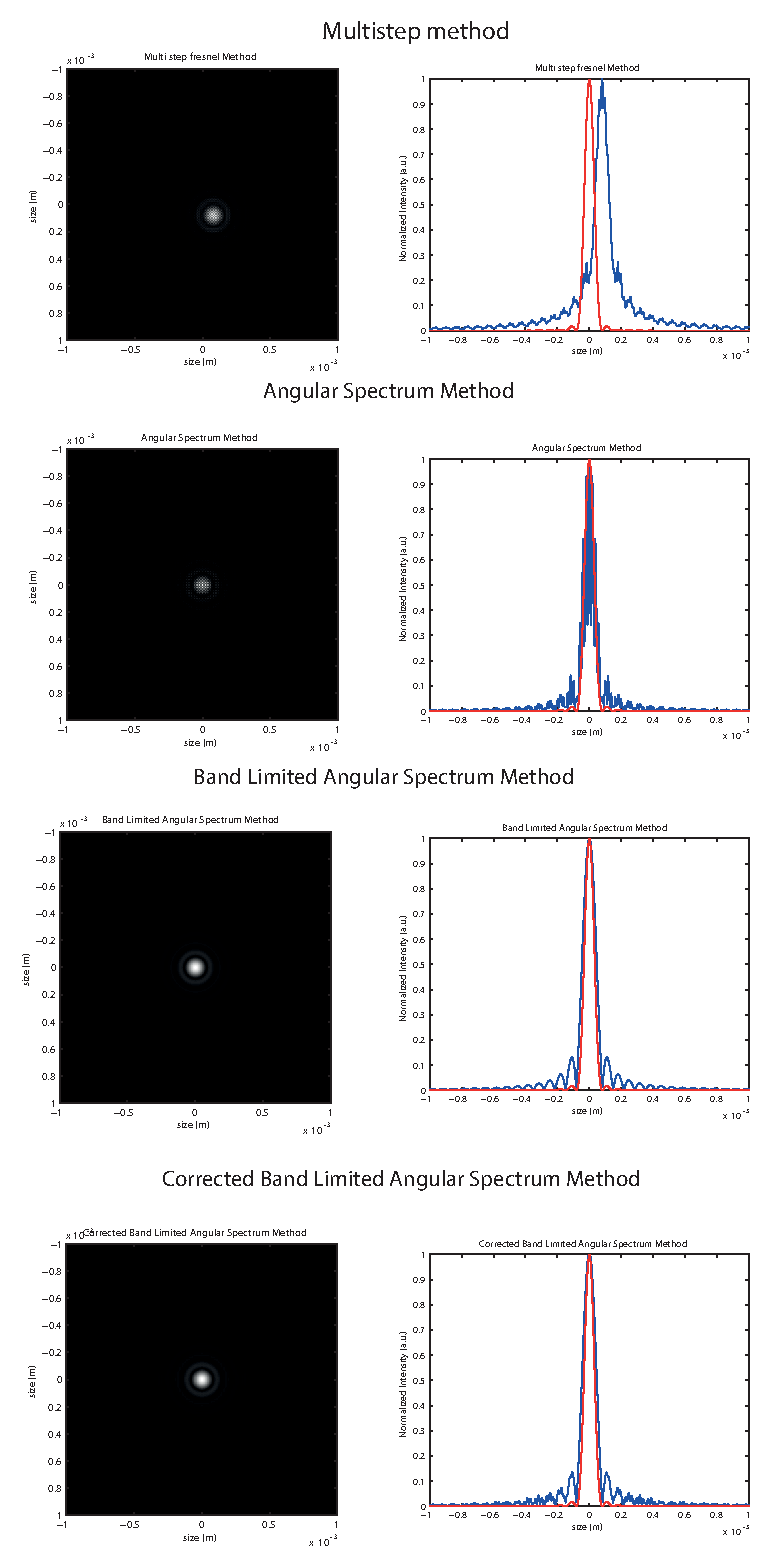
\includegraphics[height=15cm]{C:/Users/Massimo/Documents/Thesis/Thesis_PhD/methodspoint1new.eps}
	 		\end{tabular}
	 	\end{center}
	 	\caption{ \label{fig:resultspoint11} 
	 		From top to Bottom: Image and intensity cross section of a point source according to multi step method, angular spectrum method, band limited angular spectrum method and corrected band limited angular spectrum method. In red is plotted the theoretical Airy pattern for reference. }
	 \end{figure} 
	From figure \ref{fig:resultspoint11} it can be seen that in the case of the MSF method the cross section of the impulse response does not go to zero because if additive background noise. In addition to that an offset is present in the image generated. This represent a reason more to discard the multi-step method form any future simulation. The response of the AS method has a high frequency noise components superimposed to the diffraction pattern while the BL method reduces the noise due to aliasing of the transfer function in the AS case as can be seen comparing the two cross sections. Both the BL and the CBL methods present no background noise and in the high frequency noise is reduced with respect to the AS case. Another parameter to evaluate the accuracy of these methods is the position of the Airy disk first minimum. It is given by \cite{goodman2005introduction,pedrotti1993introduction}:
	 \begin{equation}
	 \label{eq:airy}
	 x_{min}=1.22\dfrac{\lambda z}{D}
	 \end{equation}
	 where $D$ is the aperture of the lens. According to the values in section \ref{sec:system} the Airy disk should have a its first minimum at $x_{min}=67 \mu m$.
	 Without considering the MSF case that is too noisy and does not present zeros, the position of the first minimum is the other cases are:\\
	 \begin {table}
	 \begin{center}
	 	\label{tab:minimum}
	 \begin{tabular}{ l | r }
	 	
	 	\hline			
	 	AS & 67.5 $\mu m$ \\
	 	BL & 77.5 $\mu m$ \\
	 	CBL & 77.5 $\mu m$ \\
	 	\hline 
	 		\end{tabular}
	 			\caption{Position of the first minimum for all the three different angular spectrum methods. }
	\end{center}
\end{table}
	As expected for both the band limited angular spectrum methods (BL and CBL) the Airy Disk is slightly wider due to the low pass filtering action that transfer function has undergone.  However noise is reduced with the band limitation as shown in figure
	 \ref{fig:resultspoint11}.
	 The noise of each diffraction patter has been estimated considering as a reference the theoretical Airy patter. After subtracting it to the calculated intensity profile, the variance has been used to estimate the noise. Values of the variance for the three different angular spectrum methods are shown in table \ref{tab:noisemethods} :
	 	 \begin {table}
	 	 \begin{center}
	 	 	\label{tab:noisemethods}
	 	 	\begin{tabular}{ l | r }
	 	 		
	 	 		\hline	
	 	 		Method & variance \\
	 	 		\hline		
	 	 		AS & 0.00120000 \\
	 	 		BL & 0.00054646 \\
	 	 		CBL & 0.00056632 \\
	 	 		\hline 
	 	 	\end{tabular}
	 	 	\caption{Noise estimation for the three different angular spectrum methods. }
	 	 \end{center}
	 	\end{table}
	 To better understand how the resolution changes with the different methods, it is worth to have a look at the Fourier transform of the images shown in figure \ref{fig:resultspoint11}. The Fourier transform of the impulse response of a system give its frequency response. The shape of the frequency response gives information about how the frequency components of the input signal are modulated and transferred to the output signal. When this function goes to zero the correspondent frequency value is called the cutoff frequency. For frequencies higher than the cutoff frequency, all the information included in the input signal is lost. Results are shown in figure \ref{fig:resultspoint2}. The graphs are symmetric with respect to the zero frequency, therefore only the positive frequencies are shown.
	 
	 \begin{figure}[h]
	 	\begin{center}
	 		\begin{tabular}{c}
	 			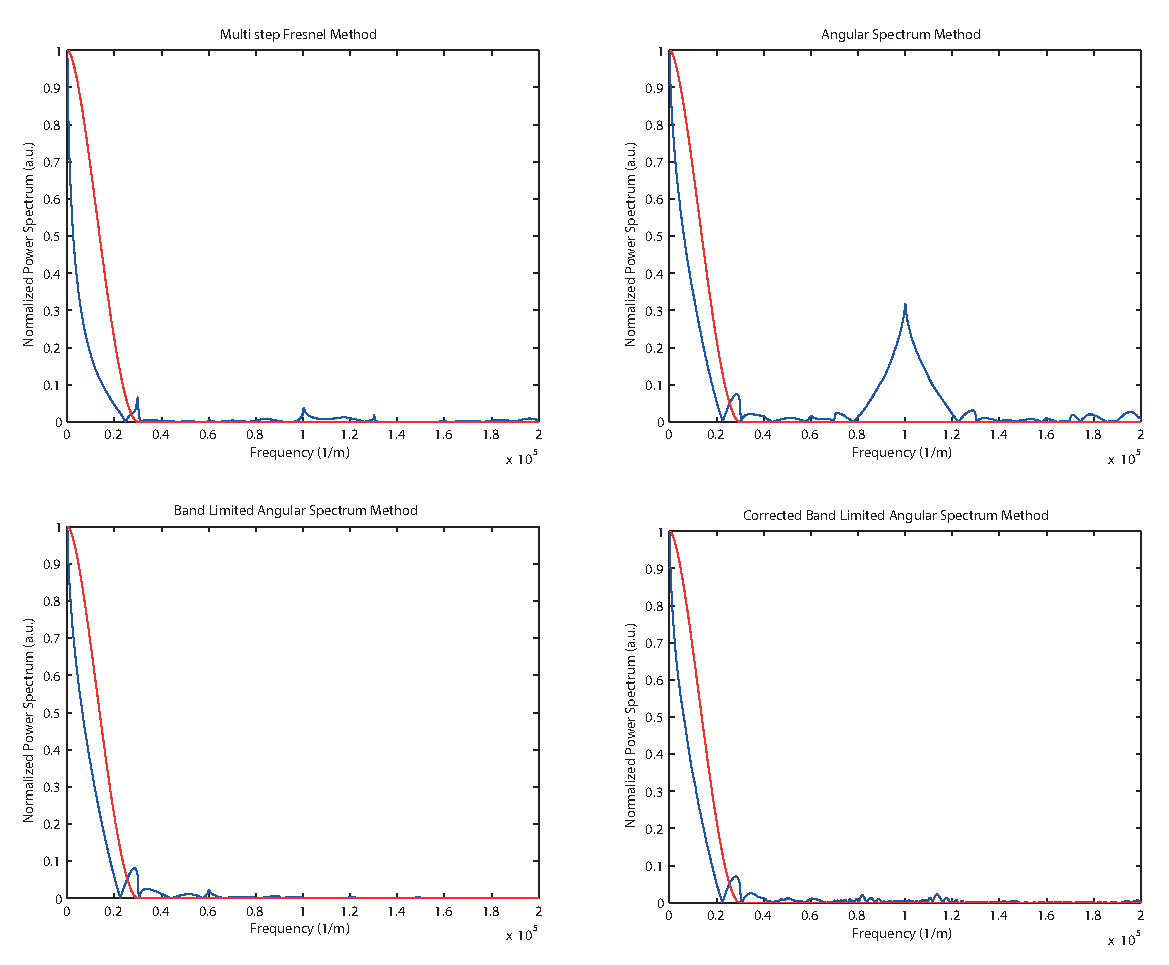
\includegraphics[height=8cm]{C:/Users/Massimo/Documents/Thesis/Thesis_PhD/MTFnew.eps}
	 		\end{tabular}
	 	\end{center}
	 	\caption{ \label{fig:resultspoint2} 
	 		From top left to bottom right: Power spectrum of the image of a point source obtained with the MSF method, the AS method, the BL method and the CBL method. In red is plotted the theoretical Airy pattern power spectrum for reference. }
	 \end{figure} 
	From a comparison of the power spectra in figure \ref{fig:resultspoint2} it is possible to note the difference in shape of the power spectrum of the MSF method, that goes to zero slower than the angular spectrum methods spectra. These three figures present as expected the same shape since for low frequency the three angular spectrum methods are identical, with the difference of the frequency components after the cut-off frequency due to the fact that the BL and the CBL have narrower bandwidths. In the AS method graph a strong peak is present at a frequency of $10^5 m^{-1}$ due to digital artefacts arising from aliasing effects. This peak disappears in the other two band limited implementations of the angular spectrum. 
	It is interesting that all four power spectra present a dispersion of the energy towards high frequencies, indicating that a noise is not avoidable in the simulation toolbox.
\section{Coherence}
\label{sec:coherence}
The Fresnel simulation toolbox has been designed to analyse a light field imaging system. Since all current and most future applications of plenoptic systems will have incoherently illuminated objects, the simulation of such a systems should take it into account. Therefore the decision to develop an algorithm to simulate light propagating in a low state of coherence was taken. In addition to that low coherent illumination avoids interference pattern cross talk between neighbours lenslets that might decrease the quality of the final image. \\
Coherence is a statistical property of light and is described in terms of second order averages known as coherence functions \cite{goodman2015statistical,mandel1995optical}. A full analysis of coherence of optical fields can be found in text books such as Born and Wolf \cite{born1999principles}, Mandel and Wolf \cite{mandel1995optical} and Goodman \cite{goodman2015statistical} and will not be discussed in this work. For the application described in this work coherence will be treated under a less rigorous point of view. Before analysing the computational model of coherence it is worth examining the two different types of coherence. As defined by Goodman \cite{goodman2015statistical} :
\begin{itemize}
	\item \textbf{Temporal Coherence} can be defined as the ability of light to interfere with a delayed version of itself
	\item \textbf{Spatial Coherence} can be defined as the ability of light to interfere with a spatially shifted version of itself
\end{itemize}
The empirical method developed to simulate light propagating at low coherence includes both spatial and temporal coherence. 
\subsection{Temporal Coherence}
\label{sec:temp}
Following the explanation of Goodman \cite{goodman2015statistical}, given a complex disturbance $U(\overrightarrow{X},t)$ with a finite bandwidth $\Delta\nu $, it is expected to remain constant during a time interval $\tau<1/\Delta\nu$. This means that the disturbance taken at two different times in the same spatial position $U(\overrightarrow{X},t)$ and $U(\overrightarrow{X},t+\tau)$ are highly correlated if $\tau<\tau_c$ where $\tau_c$ is the coherence time. Under this condition $\tau_c=1/\Delta\nu$.
Since the correlation takes place without any spatial shift it is possible to drop the spatial coordinates $\overrightarrow{X}$. The degree of temporal coherence is therefore given by the autocorrelation function:
\begin{equation}
\label{eq:coherence1}
	\Gamma(\tau) =\langle U(t+\tau)U^*(t) \rangle
\end{equation}
The coherence time $\tau$ is therefore a function of the bandwidth of the light. A perfectly monochromatic plane wave has a very narrow bandwidth and a long coherence time, while on the other hand ultra fast laser pulses will have a short coherence time and a large bandwidth. From the coherence time it is possible to define the coherence length as $l_c= v\tau_c$ where $v=c/n$ is the speed of light in the medium of propagation given by the speed of light in the vacuum $c$ divided by the refractive index $n$.
\subsection{Spatial Coherence}
To analyse spatial coherence two complex disturbances $U(\overrightarrow{X}_1,t)$ and $U(\overrightarrow{X}_2,t)$ are observed at the same time in two different position $\overrightarrow{X}_1$ and $\overrightarrow{X}_2$. When the two points coincide, $\overrightarrow{X}_1=\overrightarrow{X}_2$ the two disturbances are perfectly correlated. When the distance between the two points begins to increase, the correlation degree decreases until they become totally uncorrelated. In order to better understand this concept it is useful to illustrate the Young experiment \cite{wolf2007introduction}. With reference to figure \ref{fig:spatialcoherence} a squared light source of size $\Delta x$ emits light towards a screen at a distance R. On the screen A there are two pinholes $Q_1$ and $Q_2$. In order to have interference fringes on a second screen B the following condition should be satisfied:
\begin{equation}
\label{eq:fringes}
\Delta x \Delta \theta < \lambda
\end{equation} 
Where $2\Delta\theta$ is the angle formed at the source with the two pinholes $Q_1$ and $Q_2$ and $\lambda$ is the wavelength of the light emitted by the source. In order to see the fringes, the two pinholes should be situated in an area $\Delta A$ of size:
\begin{equation}
\label{eq:area1}
\Delta A \sim (R \Delta \theta)^2 = \dfrac{R^2}{S}\lambda
\end{equation} 
R is the distance between the screen A and the source, $S=\Delta x^2$ is the area of the source, and equation \ref{eq:fringes} has been used. The area $\Delta A$ is the coherence area of the light in the plane $A$ around the point $Q_0$ on the optical axis. 
 \begin{figure}[H]
	\centering
	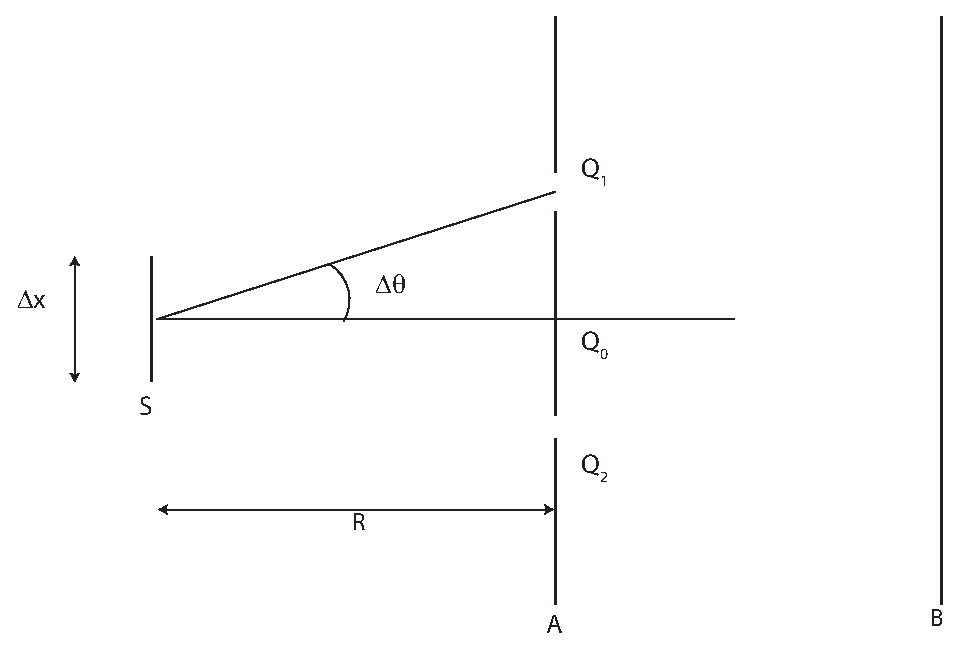
\includegraphics[width=.6\textwidth]{C:/Users/Massimo/Documents/Thesis/Thesis_PhD/spatial_coherence.eps}
	\caption{\label{fig:spatialcoherence} Young experiment setup.}
\end{figure}
The area of coherence quantifies the degree of spatial coherence. It depends on the area of the light source S, the distance of observation R and the wavelength of the light. 
\subsection{Simulation of Spatial Coherence}
\label{sec:spatial}
The goal of this section is to define a novel method for simulating spatial coherence in order to generate partially coherent optical fields. An electromagnetic wave is generated by a dipole oscillating at a certain frequency. This dipole can be a molecule, an atom, a group of atoms in a gas. In case of a conventional incandescence light source, light is emitted by tungsten atoms excited by the electrical current. This is also true for other sources of illuminations, like gas lamps, neon, or solid state light sources like LED; atoms of molecules excited to higher energy levels emit light when dropping to the ground energy level. Each dipole emits light with a certain initial phase. Considering a light source of surface $\Sigma$ containing oscillating dipoles, the elemental surfaces $d\Sigma$ is defined as the surfaces on which all the dipoles oscillate with the same phase. The average size and dimensionality of the elemental surfaces $d\Sigma$ is proportional to the degree of spatial coherence of the light source. The more coherent the light source, the bigger the elemental surfaces will be. 
From a computational point of view having a light source composed of a mosaic of surfaces with different phases is equivalent to adding a phase mask to the input field. This phase mask is composed of areas with a random phase value. The dimension of these areas gives an idea of the degree of spatial coherence. The idea behind the empirical method used to generate the phase mask is shown in figure \ref{fig:phasemask1}: 
\begin{figure}[H]
	\begin{center}
		\begin{tabular}{c}
			\includegraphics[height=7cm]{C:/Users/Massimo/Documents/Thesis/Thesis_PhD/coherence2.eps}
		\end{tabular}
	\end{center}
	\caption{ \label{fig:phasemask1} 
		A random phase mask is generated by propagating light coming form an array of sources, each one with a random phase value in the interval $[-\pi,\pi]$. }
\end{figure} 
An array of point sources is generated on a sampling window of the same dimension as the input field. The sources are placed regularly across the array. If the number of sources is less than $20 \times 20$, the sources are displaced randomly in order not to affect the coherence with their regular structure. The square root of the number of point sources used is defined as the coherence index $C$. A \textit{C} of 100 means that the initial array is composed of 100 $\times$ 100 sources. A random phase value in the range $[-\pi,\pi]$ is assigned to each of these point sources. Their amplitude is set to one. Then the array of point sources is convolved with a kernel $K$ whose size is defined in order to make all the random point sources disks of amplitude one with a finite size. All these disks touch each others without overlapping as figure \ref{fig:phasemask2} shows. The size of the kernel depends on the resolution N of the input field and on the coherence index $C$ and is equal to the ratio $N/C$.\\
The result of the convolution is a phase mask that is formed by an array of circular areas with a random phase value.
Although this array of sources is already a phase mask, it cannot be used directly in the simulation platform because of its periodicity. In fact it is not a random phase pattern. In order to randomize the shape and the distribution of the coherence areas the array of sources is propagated at a distance bigger than the size of the sources. The distance $d_c$ chosen to propagate the light sources is the one derived in section \ref{sec:fresnelmulti} to keep the same sampling both in the input and output fields using the Fresnel propagation method discussed in section. From equation \ref{eq:getz3}:
\begin{equation}
\label{eq:propcoherence}
	d_c = \dfrac{W^2}{N\lambda}
\end{equation} 
where $W$ is the field of view, $N$ is the sampling and $\lambda$ is the wavelength of the light. The choice of using the Fresnel propagation as described in section \ref{sec:Fresnel} has been made because the propagation distance is small and hence aliasing issues do not arise. In addition to that it only requires one Fourier transform, making the random phase generation algorithm faster.
The whole process is shown in figure \ref{fig:phasemask2}
\newpage
\begin{figure}[H]
	\begin{center}
		\begin{tabular}{c}
			\includegraphics[height=15cm]{C:/Users/Massimo/Documents/Thesis/Thesis_PhD/phasetarray200.eps}
		\end{tabular}
	\end{center}
	\caption	{ \label{fig:phasemask2} 
		Process of the creation of the phase mask. Top: array of point sources with a random phase value; centre: array of the areas of coherence at source after the convolution with $K$; bottom: randomized areas of coherence at object plane after the propagation of $d_c$. }
\end{figure} 
Some examples of phase masks generated from different number of sources can be seen in figure \ref{fig:phasemask3}:
\begin{figure}[H]
	\begin{center}
		\begin{tabular}{c}
			\includegraphics[height=15cm]{C:/Users/Massimo/Documents/Thesis/Thesis_PhD/phi.eps}
		\end{tabular}
	\end{center}
	\caption{ \label{fig:phasemask3} 
		Final random phase mask generated a coherence index C equals to 10, 50, 100 and 200. }
\end{figure} 
The algorithm to generate the random phase mask can be summarized as follow:
\begin{itemize}
\item A number of light sources are defined, arranged in a regular array and allocated a random phase between $-\pi$ and $\pi$. 
 \item Each source has a size diameter given by: $N/C$
 \item This array of sources is then propagated a distance $d_c$ shown in equation \ref{eq:propcoherence} in order to randomize the shape of the coherence areas.
 \item the resultant phase is used as the output phase mask to add the input field.
\end{itemize}
These considerations lead to correct results as proven by the simulation of the image of an edge presented in section \ref{sec:coherencevsinco}.
\newpage
\subsection{Simulation of Temporal Coherence}
\label{sec:simtempcoherence}
 As discussed in section \ref{sec:temp}, temporal coherence is defined by the time $\tau$ in which the optical wave is correlated with itself. In other words after a time $t=\tau$, the optical disturbance $U(t)$ and $U(t+\tau)$ are totally uncorrelated and cannot interfere with each other. 
To simulate this effect many snapshots of the output field are taken each time using a different random distribution of phases for the sources. Assuming that the time difference between every snapshot is larger than or equal to the coherence time $\tau$. For the application for which this toolbox has been designed it is not relevant to know the exact value of $\tau$. However, the light source used for the laboratory prototype, that will be described in chapter \ref{chap:microscope}, was a Thorlabs LED Array Light Source LIU630A with a wavelength centred on 630 nm and a bandwidth $\Delta\lambda=20 nm$. The emission spectrum is shown in figure \ref{fig:emission_spectrum}.
\begin{figure}[H]
	\begin{center}
		\begin{tabular}{c}
			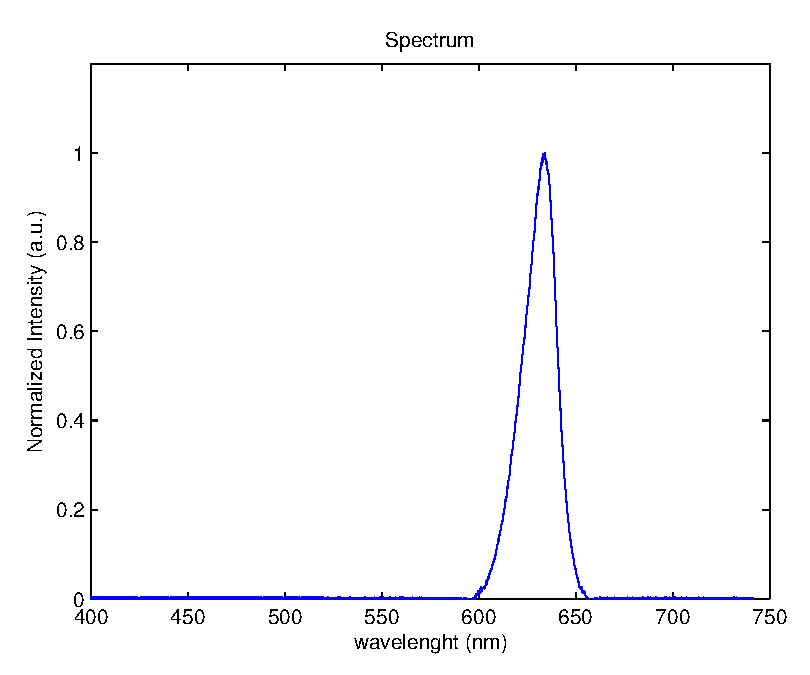
\includegraphics[height=7cm]{C:/Users/Massimo/Documents/Thesis/Thesis_PhD/spectralLED.eps}
		\end{tabular}
	\end{center}
	\caption{ \label{fig:emission_spectrum} 
		Emission spectrum of the LED considered in our simulations and real image system. Data plotted from Thorlabs LED Array Light Source LIU630A datasheet. }
\end{figure} 
 Its coherence time is given by:
\begin{equation}
\label{key}
\tau = \dfrac{1}{\Delta\nu}=\dfrac{\Delta\lambda}{c}
\end{equation}
which is equal to $\tau=6.6\times10^{-17} s$. 
 Therefore each snapshot is assumed to be taken at the image plane at an interval of $\tau$. 
 All the snapshots are then added together, integrating the optical disturbance over time. Longer integration times will give better contrast and less noise while approaching to the incoherent imaging as it is shown in the following paragraph.
 \section{Optimization of Coherence Parameters}
 In this section simulation will be presented in order to estimate the best values of the simulation parameters to produce partially coherent light. These parameters are the coherence coefficient $C$ for spatial coherence and the number of snapshots for the temporal coherence. A resolution target was imaged by a 2f system described in section \ref{sec:system}.
 \subsection{Optimization of Spatial Coherence}
 Simulations have been run propagating an optical disturbance with phase masks generated with different values of the parameter \textit{C} with the purpose of defining the optimal number of sources to generate a phase mask that produces a final images with a high signal to noise ratio.
 The input field used is the USAF resolution target, shown in figure \ref{fig:USAF}
 \begin{figure}[H]
 	\begin{center}
 		\begin{tabular}{c}
 			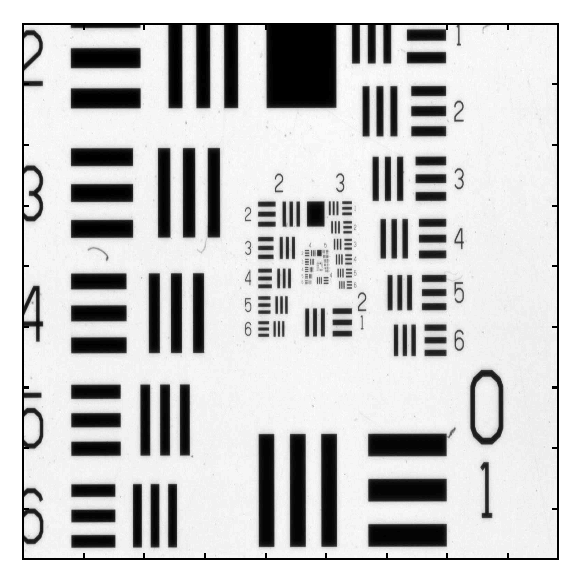
\includegraphics[height=3cm]{C:/Users/Massimo/Documents/Thesis/Thesis_PhD/USAF.eps}
 		\end{tabular}
 	\end{center}
 	\caption{ \label{fig:USAF} 
 		USAF resolution target. }
 \end{figure} 
 The first simulation has been made changing the coherence index $C$ from a value of 5 (high coherence) to 500 (low coherence) in a sampling window with a resolution of 1765 by 1765 pixels.
 Figure \ref{fig:spatialsnr2} shows how the field at the image plane for different values of \textit{C} appears, while figure \ref{fig:spatialsnr1} shows a plot of the signal to noise ratio of the images as a function of the coherence index showing an asymptotic behaviour. After a certain threshold value of $C$, increasing the coherence index does not improve the image quality. The threshold is defined as the value of $C$ for which the variance of the previous five values of SNR is less than 0.01.
 Figure \ref{fig:spatialsnr1} shows that for values of $C$ bigger than 250 the SNR asymptotically tends to 18 dB. In this case the resolution of the input field, and therefore of the phase mask, is 1765 by 1765 pixels, so that the SNR reaches the asymptote when the ratio between the number of sources and the resolution is 0.14. After this point, there is no gain in making the light source more incoherent in terms of signal to noise ratio improvement.
 \begin{figure}[H]
 	\centering
 	\includegraphics[width=.4\textwidth]{C:/Users/Massimo/Documents/Thesis/Thesis_PhD/iota.eps}
 	\caption{\label{fig:spatialsnr2}Images of the USAF resolution target with different values of $\iota$. Increasing the number of point sources generating the phase mask leads to more incoherent imaging, leading to improved resolution. Images where obtained with 300 iterations.}
 \end{figure}
 The ratio between the number of sources \textit{C} and the resolution of the optical field \textit{N} is defined as the incoherence degree $\iota$:
 \begin{equation}
 \label{eq:incoherence_degree}
 \iota = \dfrac{C}{N}
 \end{equation}
 \newpage
 
 \begin{figure}[H]
 	\centering
 	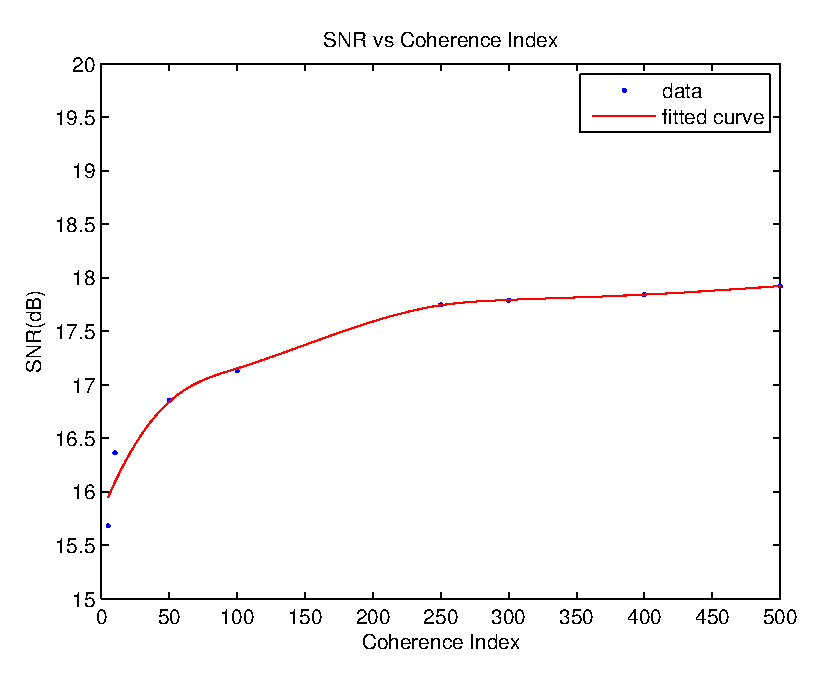
\includegraphics[width=1\textwidth]{C:/Users/Massimo/Documents/Thesis/Thesis_PhD/SNRspatial.eps}
 	\caption{\label{fig:spatialsnr1}Signal to noise ratio of the image of a USAF resolution target plotted as a function of the coherence index $C$.}
 \end{figure}
 The image quality evaluated using the signal to noise ratio improves with the increasing of the sources used to generate the phase mask. However it reaches an asymptote after 250 sources. This is due to the fact that the interference effects due to low coherence decrease, improving image quality. 
 \newpage
 \subsection{Optimization of Temporal Coherence}
The second simulation run aimed to define the investigate the effect of increasing the number of snapshots on temporal coherence effects. The random phase mask acts as a diffuser, and the resultant output field obtained by a single snapshot will present a low signal to noise ratio due to speckles, as shown in figure \ref{fig:speckle}
\begin{figure}[H]
	\centering
	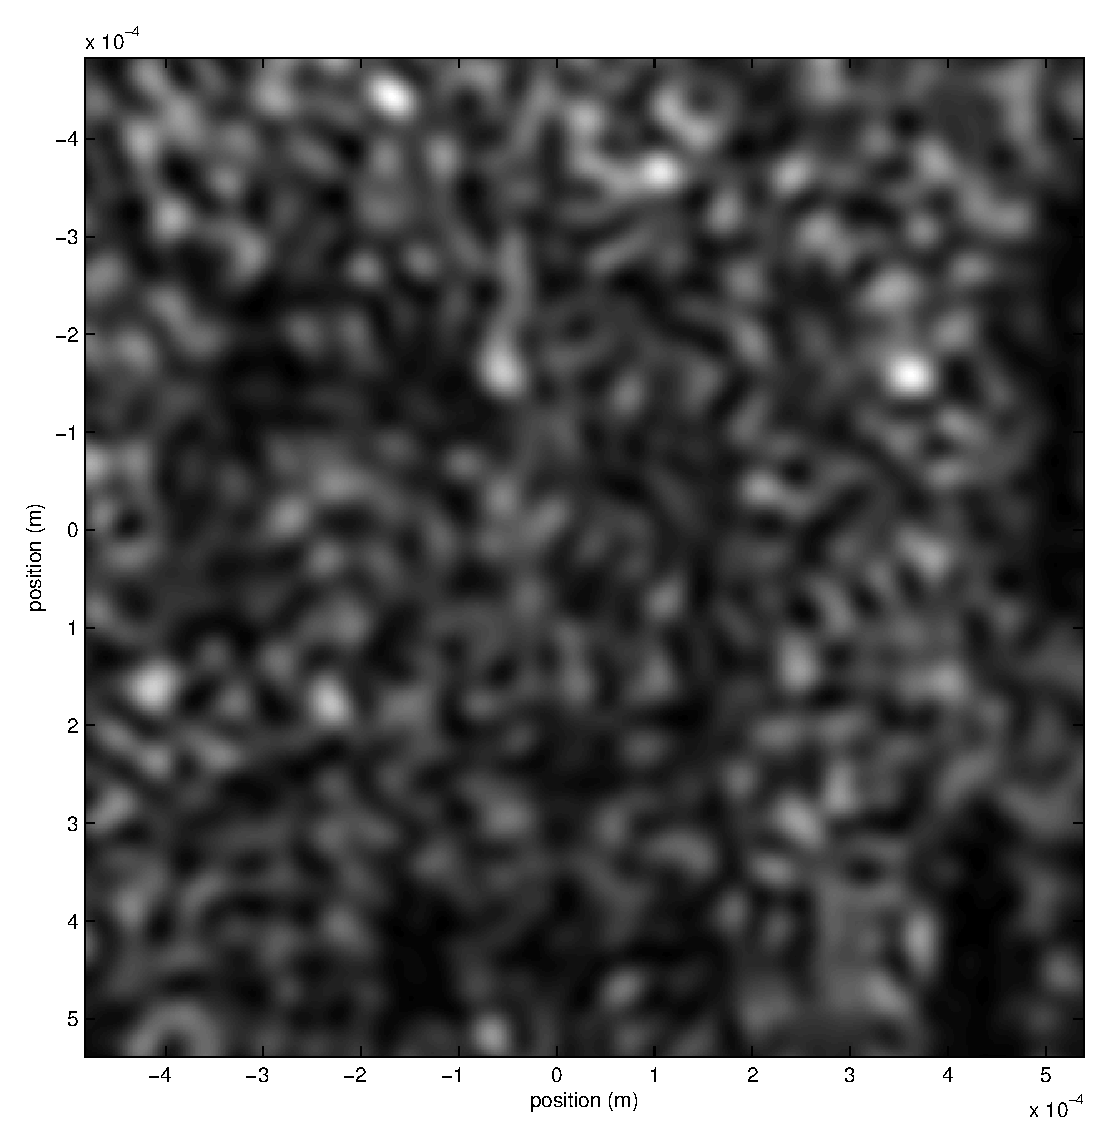
\includegraphics[width=.5\textwidth]{C:/Users/Massimo/Documents/Thesis/Thesis_PhD/USAF5iter.eps}
	\caption{\label{fig:speckle}Noise due to the speckles in an image of a USAF resolution target after only 5 snapshots.}
\end{figure}
Taking several snapshots and adding them all together is equal to an integration over time of the optical field reaching the sensor. While increasing the integration time, the noise due to the speckles drops considerably. Figure \ref{fig:iter} shows several images of the USAF target in figure \ref{fig:USAF} taken with an incoherence degree of $\iota=0.14$, and with an increasing number of snapshots from 5 to 1000.
 \begin{figure}[H]
 	\centering
 	\includegraphics[width=1\textwidth]{C:/Users/Massimo/Documents/Thesis/Thesis_PhD/iter.eps}
 	\caption{\label{fig:iter}Images of the USAF resolution target obtained adding an increasing number of snapshot. this is equivalent to increase the integration time of the sensor. The noise due to the speckles caused by the phase mask decreases with increasing number of snapshots. images are obtained summing the snapshots, therefore they do not have the same brightness.}
 \end{figure}
 Since increasing the number of snapshots is computationally expensive, the signal to noise ratio of the images in figure \ref{fig:iter} has been evaluated and plotted as a function of the number of snapshots in order to define an optimal parameter. Results are shown in figure \ref{fig:SNRiter}. The threshold is defined as the number of snapshots for which the variance of the previous five values of SNR is less then 0.01.
 \begin{figure}[H]
 	\centering
 	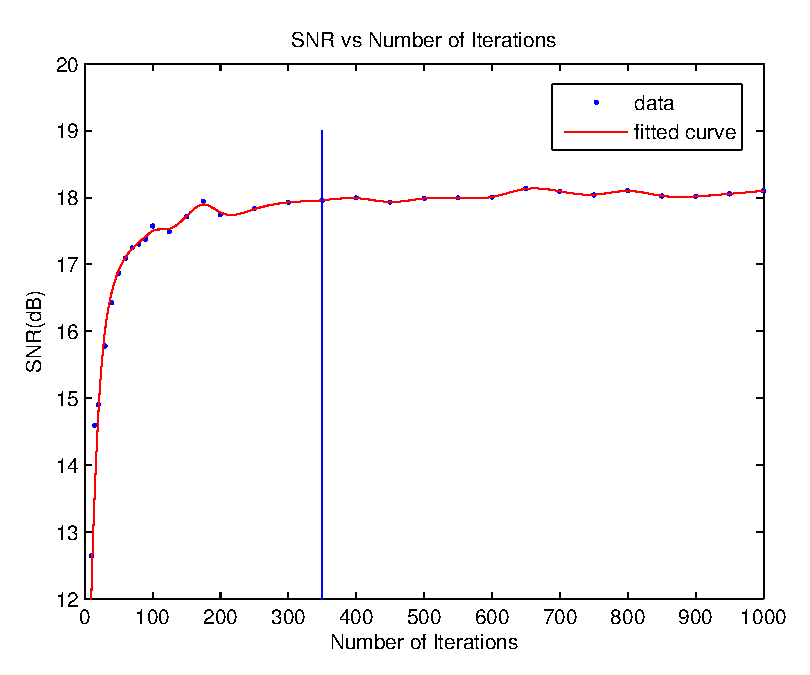
\includegraphics[width=1\textwidth]{C:/Users/Massimo/Documents/Thesis/Thesis_PhD/SNRtemporal.eps}
 	\caption{\label{fig:SNRiter}Signal to noise ratio as a function of the number of iterations. The threshold has been calculated looking at the variance of the previous five data. The purpose of the fitted curve is to show the asymptotic behaviour of the data.}
 \end{figure}
 For an image with an incoherence degree of $\iota=0.14$ the number of iterations after which the SNR of the image does not improve further is 350. After that value the SNR tends asymptotically to 18 dB in spite of an increased computational effort. Therefore from a SNR point of view the optimal number of iteration to simulate temporal incoherence is 350. All the other simulations presented in this work will be performed with the coherence parameters discussed in this section. 
\subsection{Coherent Imaging vs Incoherent Imaging}
\label{sec:coherencevsinco}
The image of an edge has been simulated to make a comparison between the coherent and the incoherent system response. Data were simulated with the same optical parameters described in section \ref{sec:system}. The intensity profile of an image of an edge is well known both in the case of coherent and incoherent illumination and provides a means of verification for the simulation methodology discussed above. Figure \ref{fig:coherenceprofile} shows the response of a coherent and an incoherent imaging systems to a sharp edge. The intensity profile of the edge is shown in green, its coherent image in blue and the incoherent image is shown in red. The coherent image presents fringes whose amplitude decreases further away from the edge. This effect is known as ringing artefacts, due to the coherent transfer function that usually presents rapid discontinuities \cite{goodman2005introduction}. Another property of the coherent image is that it crosses the actual location of the edge at 1/4 of its asymptotic value of intensity, while the incoherent image does the same at 1/2 of its asymptotic value, as can be seen in figure \ref{fig:coherenceprofile} \cite{goodman2005introduction}. Both conditions are verified by the simulations run as shown in figure \ref{fig:coherenceprofile}. \\
\\
\\
\begin{figure}[H]
	\centering
	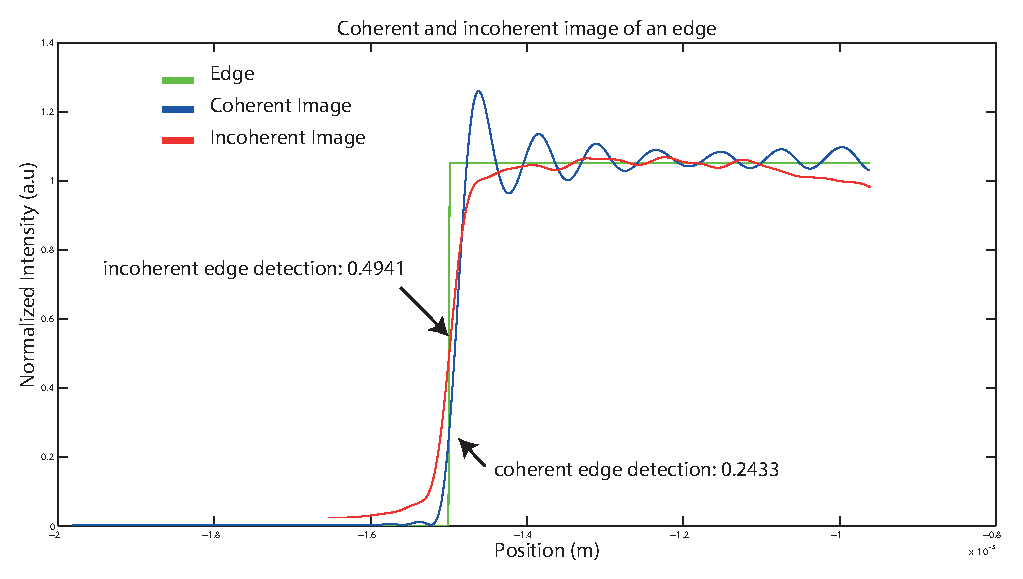
\includegraphics[width=.9\textwidth]{C:/Users/Massimo/Documents/Thesis/Thesis_PhD/2dedge.eps}
	\caption{\label{fig:coherenceprofile}Comparison between the coherent and an incoherent response of a simple 2f system to a sharp edge.}
\end{figure}
\section{Conclusions}
In this  chapter it was shown how the methods described in chapter \ref{chap:fresnel} can be implemented by the simulation toolbox. A comparison between the different free space propagation methods described in chapter \ref{chap:fresnel} was presented in section \ref{sec:perfAS} showing how the corrected band limited angular spectrum method is the most suitable to simulate an imaging system since presents the best trade-off between computational performance, Signal to Noise ration and accuracy of the output field. This has been proven further in section \ref{sec:comp} where the image of a point source obtained with the four different method has been analysed both in the spatial and frequency domain. \\
The last two sections of this chapter discuss coherence and present an original method to simulate partially coherent light sources. The method is described in details and an estimation of the best simulation parameters is presented. The correctness of the results is proven through the simulation of an infinite edge presented in section \ref{sec:coherencevsinco}. 
\nomenclature{$\overrightarrow{E}$}{Electric field}
\nomenclature{$\overrightarrow{H}$}{Magnetic field}
\nomenclature{$\epsilon$}{Electrical permittivity}
\nomenclature{$\mu$}{Magnetic permittivity}
\nomenclature{$\nabla$}{Laplacian operator}
\nomenclature{$\widehat{i},\widehat{j}$, $\widehat{k}$}{unit vectors}
\nomenclature{$n$}{Refractive index}
\nomenclature{$c$}{Speed of light in vacuum}
\nomenclature{$t$}{Time}
\nomenclature{$u$}{Field disturbance}
\nomenclature{$\nu$}{Optical frequency}
\nomenclature{$\phi$}{Phase}
\nomenclature{$k$}{Wave number}
\nomenclature{$U$}{Complex field}
\nomenclature{$\eta, \chi$}{Object space coordinates}
\nomenclature{$\sigma$}{Area of the aperture}
\nomenclature{$f_x, f_y$}{Spatial frequencies}
\nomenclature{$\nu_x, \nu_y$}{Local spatial frequencies}
\nomenclature{SNR}{Signal to noise ratio}
\nomenclature{$\Delta$}{Thickness function}
\nomenclature{$t_{lens}$}{Transmission of the lens}
\nomenclature{R}{Radius of curvature of a lens surface}
\nomenclature{$N$}{Number of samples}
\nomenclature{$r$}{Radius of a lens aperture}
\nomenclature{$F_\#$}{F-number}
\nomenclature{$\nu_c$}{Optical cut-off frequency}
\nomenclature{$x_{min}$}{Position of Airy Disk first minimum}
\nomenclature{$\Gamma$}{Autocorrelation function}
\nomenclature{$\tau$}{Coherence time}
\nomenclature{$A$}{Area}
\nomenclature{$\Delta S$}{Area of the emitting source}
\nomenclature{$d\Sigma$}{Elemental area}
\nomenclature{$C$}{Coherence index}
\nomenclature{$d_c$}{Distance of propagation in the coherence algorithm}
\nomenclature{$W$}{Size of the input optical field}
\nomenclature{$\iota$}{Incoherence degree}

